In the last decades, the formalization of mathematical knowledge (and the verification and automation of formal proofs) has become of ever increasing interest. Formal methods nowadays are not just used by computer scientists to verify software and hardware as well as in program synthesis, but -- due to problems such as Kepler's conjecture \cite{HalAdaBau:afpkc15}, the classification theorem for finite simple groups \cite{Solomon:fsgc95}, etc. -- are also becoming increasingly popular among mathematicians in general. 

By now, there is a vast plurality of formal systems and corresponding libraries to choose from. However, almost all of these are non-interoperable, because they are based on differing, mutually incompatible logical foundations (e.g. set theories, higher-order logic, variants of type theory etc.), library formats, library structures, and much work is spent developing the respective basic libraries in each system.

Moreover, since a library in one such system is not reusable in another system, developers are forced to spend an enormous amount of time and energy developing basic library organization features such as distribution, browsing/search or change management for each library format; all of which binds resources that could be used to improve core functionality and library contents instead.\medskip

One reason for the incompatibility is the widespread usage of the \emph{homogeneous method}\footnote{The terminology \emph{homogeneous/heterogeneous} is due to Florian Rabe, unpublished.}, which fixes some logical foundation with all primitive notions (e.g. types, axioms, inference rules) and uses conservative extensions of this foundation to allow for modeling some specific domain knowledge. 
While homogeneous reasoning is conveniently implementable and verifiable, it implies that a lot of work is needed just to model the basic domains of discourse necessary for mathematics, such as real numbers, algebraic theories, etc. Moreover, the resulting formalizations are actually less valuable to mathematicians, since they are intimately dependent on (and framed in terms of) the underlying logic, making it virtually impossible to move the results between different foundations or to abstract from them. 

In contrast, mathematical practice favors the \emph{heterogeneous method}, as exemplified by the works of Bourbaki \cite{bourbakiunivers}. In heterogeneous reasoning, theories are used to introduce new primitive notions and the truth of some proposition is relative to a theory (as opposed to absolute with respect to some foundation). This method is closely related to the ``little theories'' paradigm \cite{littletheories} which prefers to state each theorem in the weakest possible theory, thus optimizing reusability of mathematical results.
Even though in theory, all of mathematics can be reduced to first principles -- most prominently first-order logic with (some extension of) ZFC -- it is usually carried out in a highly abstract setting that hides the foundation, often rendering it irrelevant and thus allowing it to be ignored. \medskip

Correspondingly, there is an inconvenient discrepancy between the currently existing formal libraries and the way (informal) mathematics is usually done in practice. Furthermore, the available formal knowledge is distributed among dozens of different mutually incompatible formal library systems with considerable overlap between them. 

\paragraph{} Additionally, \cite{CarFarKohRab:bmobb19} recently introduced the \emph{five aspects of big math systems} -- aspects of doing mathematics that can and should be supported by software, collectively referred to as \emph{tetrapod}, as in \autoref{fig:tetrapods}. These aspects are
\begin{enumerate}
	\item \emph{inference} as supported by interactive and automated proof systems, 
	\item \emph{computation} as supported e.g. by computer algebra systems, 
	\item \emph{tabulation} as e.g. supported by databases of mathematical objects (finite groups, graphs, etc.) and their properties, 
	\item \emph{narration} as supported e.g. by \LaTeX\ and other text formating software with strong support for mathematical expressions, and finally 
	\item \emph{organization} of formal knowledge.
\end{enumerate}

\begin{figure}[ht]\centering
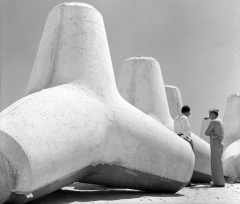
\includegraphics[width=5.5cm]{img/tetrapod}\qquad\qquad
\input{img/tetrapod-arms}
\caption{Tetrapods: Real and  Conceptual}\label{fig:tetrapods}
\end{figure}

Most software systems focus on one of those tetrapod aspects, few on two, and none strongly support all of them. That is despite the fact that all five of these aspects are intrinsic and important parts of doing real-world mathematics, and it is correspondingly vital to support all of them in an interconnected workflow.

What we should consequently aim for is a \emph{universal archiving solution for all formal knowledge}, that
\begin{enumerate}
	\item does not depend on a specific logical foundation, 
	\item can import libraries from different formal systems, allowing one to choose which system to use
		for generating new content, 
	\item allows for abstracting from and transferring results between differing foundations and library 
		structures,
	\item supports all five aspects of big math systems.
\end{enumerate}

The aim of this thesis is to describe our approach to achieving such an archiving solution by integrating the libraries of existing software systems, focusing on the \emph{inference}, \emph{computation}, \emph{tabulation} and \emph{organization} aspects of the tetrapod, and to demonstrate its feasibility.
